% Copyright 2008 Markus Kohm
% 
% This work may be distributed and/or modified under the
% conditions of the LaTeX Project Public License, either version 1.3
% of this license or (at your option) any later version.
% The latest version of this license is in
% http://www.latex-project.org/lppl.txt
% and version 1.3 or later is part of all distributions of LaTeX
% version 2005/12/01 or later.
% 
% This work has the LPPL maintenance status `maintained'.
% 
% The Current Maintainer of this work is Markus Kohm.
% 
% This work consists of this file only.
%-----------------------------------------------------------------------
\documentclass[parskip=half, a4paper, DIV=14]{scrartcl}

\usepackage[ngerman,english]{babel}
\usepackage{helvet}
\usepackage{graphicx}
\usepackage{layout}

%http://de.wikibooks.org/wiki/LaTeX-W%C3%B6rterbuch:_fontfamily
\renewcommand{\familydefault}{\sfdefault}
\fontfamily{phv}\selectfont

\begin{document}

\title{Database System Project (SS 2015)}
\subtitle{MyMeal -- System requirement report}
\author{Saulo Ribeiro de Andrade -- 7120309033\\
		Alexander Goscinski -- 7120309027\\
		Christan Würthner -- c.wuerthner@me.com}
\date{\today}
\maketitle


\section{Functional specification}
Our project is an implementation of a food delivery system called MyMeal accessible as
a web page. It offers important features like 
searching for restaurants and for food available for ordering, or an ordering
process for customers. We have three kinds of user in our system: visitor, customer and restaurant.
A visitor is a person visiting our web page having no session id. A customer is already a
registered user with the possibility to order food. A restaurant is also a
registered user, who represents the restaurant with its menu.

\begin{figure}[hb]
	\centering
		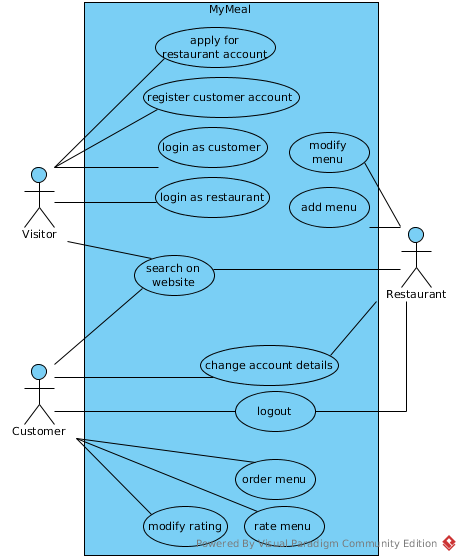
\includegraphics[scale=0.7]{UseCaseDiagramHunger.png}
	\caption{Use case diagram of our system.}
\end{figure}


A visitor of our website can search on it, log in as a customer or
as a restaurant, register an customer account and also apply for a restaurant account.
For now the application of a restaurant account will be processed by our similar to the
registration of a customer account. That means every restaurant will be accepted.
The application process is an optional goal.

An user logged in as a customer has the following possibilities: search
for restaurants or menus, rate a menu after it was
delivered, modify his/her rating his rating, modifying account details and
order a menu.

An user logged in as a restaurant will be able to add and modify 
his/her menus as well as the restaurant's account details 
and will also be able to search for restaurants or menus.

Optional goals: An application process for the restaurants, with 
approvement of an additional kind of user with administrative rights.
The option for a restaurant to accept or cancel an order.
The option for a customer to cancel a yet non accepted offer.
In addition we would like to offer an recommendation system for the customers based on the customer's
previous orders and ratings using machine learning techniques like neural networks
and gradient boosting.

\section{Technical specification}
The Server will run on python. We use the Rest interface for communication
between front and back end. For the front end we use HTML, Javascript and CSS in addition with commonly used frameworks
The database will run on MySQL.

\section{Used frameworks}
Front end:\\
Bootstrap (CSS)\\
jQuery (JavaScript)

Back end:\\
Eve (Python)\\
scikit-learn (Python, optional)
\end{document}



